\documentclass[letterpaper,12pt]{texMemo}

\usepackage{graphicx}

\memoto{The School House Board of Managers}
\memofrom{The School House Sand \& Salt Committee}
\memosubject{Winter Closeout}
\memodate{Sunday, March 29, 2020}
% \memologo{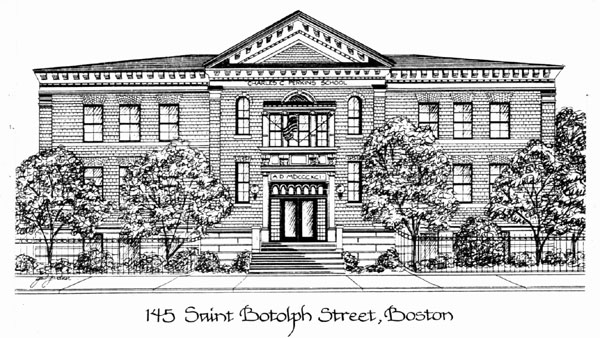
\includegraphics[height=8\baselineskip]{schoolhouse-etching.jpg}}
% \logo{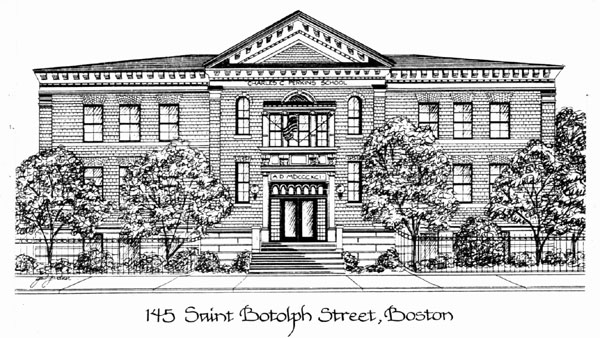
\includegraphics[width=0.3\textwidth]{schoolhouse-etching.jpg}}

% Add vertical space between paragraphs
\setlength{\parskip}{\baselineskip}

\begin{document}
\maketitle

It is time to bid our mild 2020 winter adieu. Sand, salt, and shovels
have been stowed in the building storeroom until winter weather
returns in late 2020.  We had little in the way of snow and ice this
winter, making a light load for the sand and salt supplies near the
front and parking lot doors. Supplies were checked periodically
throughout the winter and replenished as needed.

The mild winter brought a substantial cost savings to The School House
as well. Due to the mild conditions, The Sand \& Salt Committee had no
expenditures. We thank The School House Board of Managers for allowing
us to incorporate this savings into our annual off-site celebration
weekend. Sadly, the planned boat cruise must be postponed due to the
Coronavirus.

\begin{table}[h]
\centering
\begin{tabular}{lll}
      & 2019    & 2020   \\
Sand  & \$3.67  & \$0.00 \\
Salt  & \$40.31 & \$0.00 \\
Other & \$10.04 & \$0.00 \\ \cline{2-3} 
Total & \$54.02 & \$0.00
\end{tabular}
\caption{Sand \& Salt Expenditures}
\label{tab:my-table}
\end{table}

\end{document}
